\chapter{General discussion}
\label{discussion}

\section{Introduction}

This chapter provides a general discussion about the experiments and findings in this study. Specially, both theoretic and practical implications of the current study will be introduced. The first section will focus on how the current study contributes to L2 speech learning theories, and the second section will focus on how the current study contributes to automatic accentedness evaluation.

\section{Implication for L2 speech learning theories}

As reviewed in chapter \ref{literature}, a bunch of studies have investigate the effect of L1 in the acquisition of L2 phonological properties. This effect presents in both segmental (as shown by \cite{strange1992learning, flege1987production, chang2008phonetic, munro1993productions, derakhshan2015interference}) and suprasegmental acquisition (as shown by \cite{mennen2004bi, stockmal2005measures, white2007calibrating, lin2008interlanguage, li2014l2, ordin2015acquisition}). However, for segmental properties acquisition, almost all previously mentioned studies have several limitations to comprehensively reveal the detail about the L1's effect on L2 acquisition:

\begin{enumerate}
\item Almost all studies only focus on a specific phonological phenomenon, and analyze how L1 affect the production in L2.
\item Usually the numbers of analyzed speakers and L1s are quite limited.
\item Those studies can only show the L1's effect exist, but there is no way to quantize the influence of L1.
\item Few studies investigate the relationship between L1's effect and degree of foreign accent.
\end{enumerate}

For suprasegmental properties acquisition, thanks to the study by \cite{ramus1999correlates,grabe2002durational}, several publications use durational rhythmic measurements to show the change of those measurements at different stage of L2 learning. However, these studies still have the similar limitations that the numbers of L1s and speakers per L1 are small. Moreover, no quantified speakers' accentedness scores are available in those studies, only some qualitative ranges (for example, from beginners to advanced learners).

Different from the methodology presented in previous work, the current study proposes to use a computational framework to quantify the L2 speech learning outcomes of tens of speakers from multiple L1s. Both segmental and suprasegmental phonology acquisition are investigated. The analyses done in this study further validate that the influence of L1 exists in both segmental and suprasegmental phonology acquisition during L2 learning. More importantly, with the L1s' information, multiple regression analysis reveals that the accentedness can be better explained. Besides this, the current study further shows that the difference originates from speakers' L1s will also be presented in their accented speech through the analysis of relative importance of segmental and suprasegmental features to accentedness scores. In the following, Mandarin speakers will be taken as examples to illustrate how the methodology proposed by this study can be further utilized to investigate the L2 speech learning process.

\begin{figure}[t]
        \begin{minipage}[t]{1.0\linewidth}
        \centering
            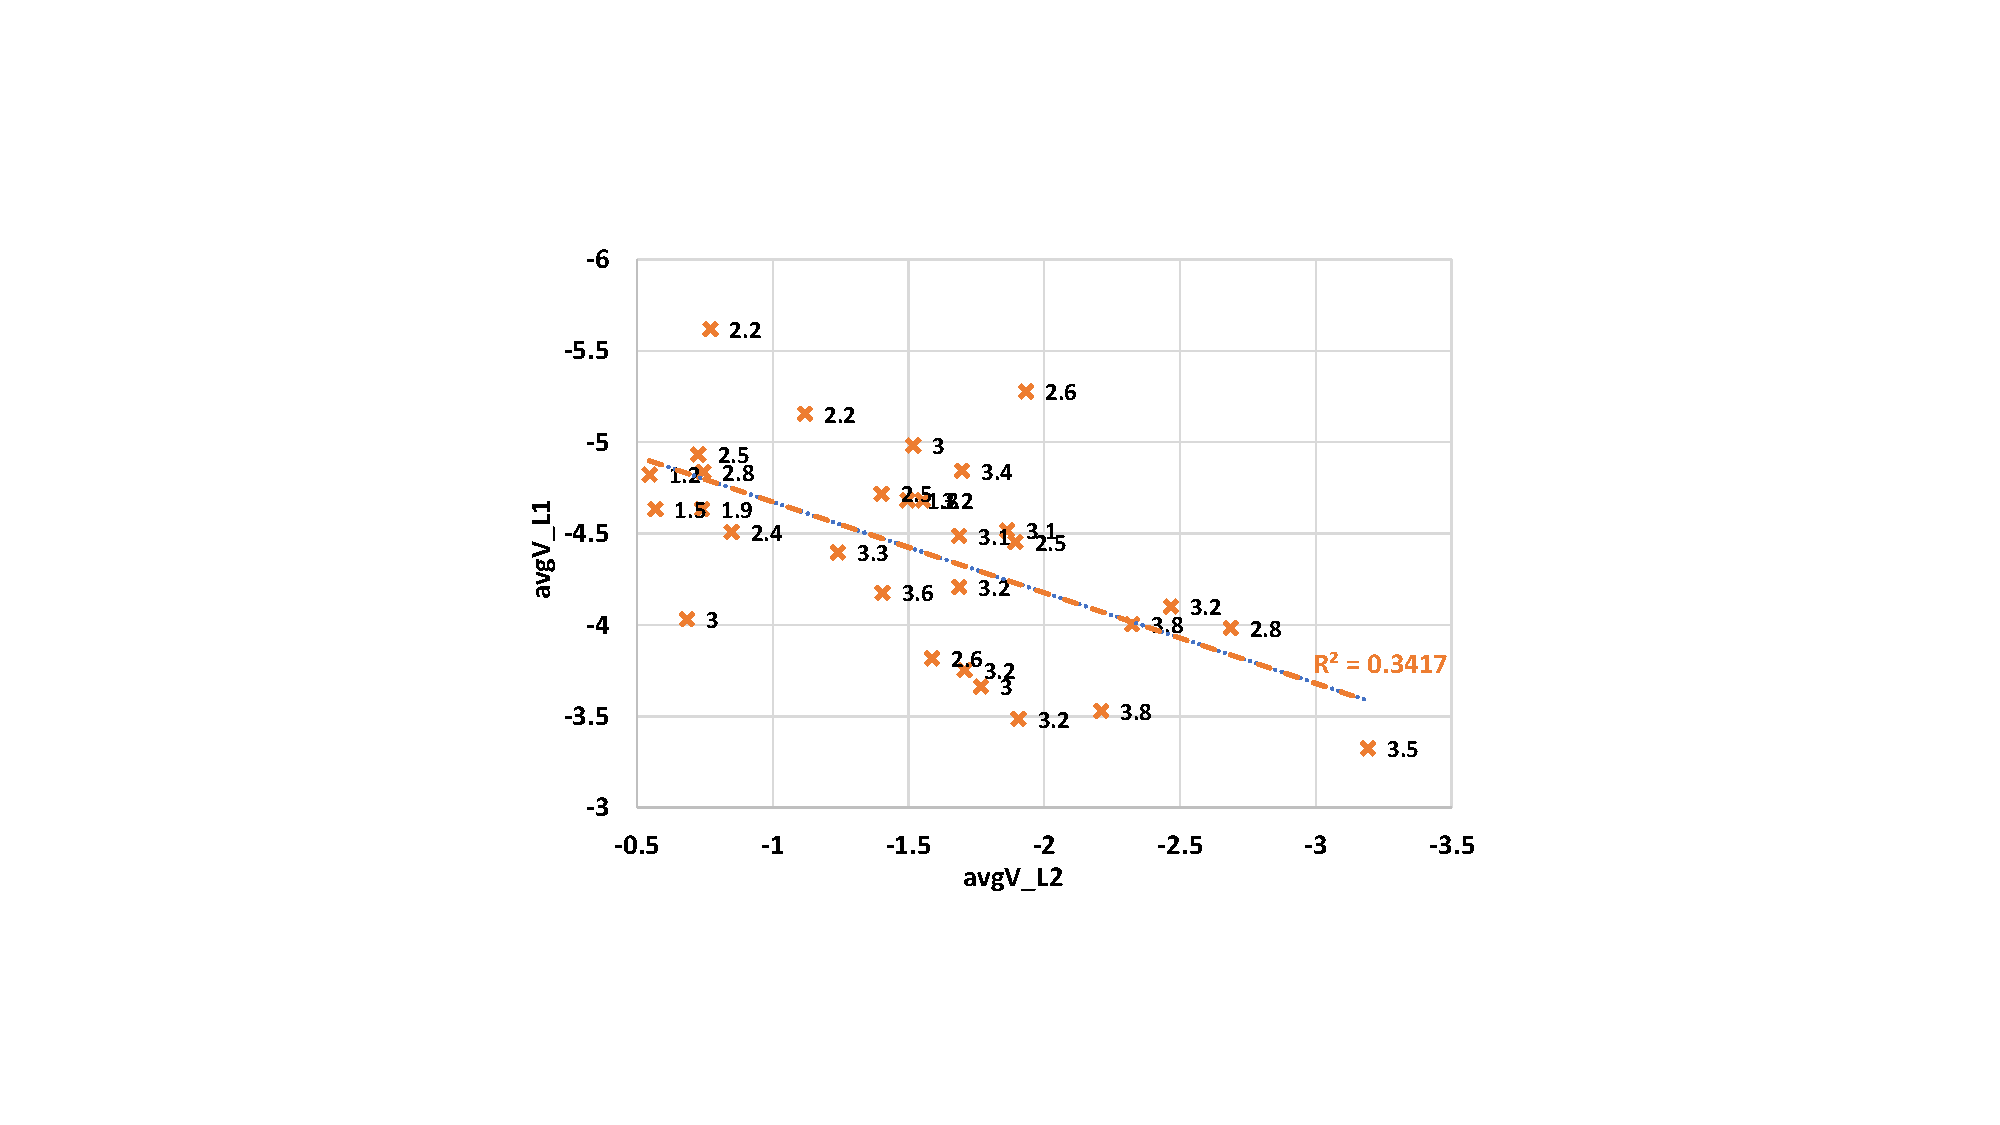
\includegraphics[width=5.0in]{figures/ch7_seg.pdf}
        \end{minipage}%
        \caption{The average pronunciation scores of vowels in accented speech by Mandarin speakers using both L2 (X-axis) and L1 (Y-axis) acoustic models. Larger pronunciation score means closer vowel pronunciation to the pronunciation pattern defined by corresponding acoustic model.}
        \centering
        \label{fig:ch7_seg}
     \end{figure}

Figure \ref{fig:ch7_seg} shows the average pronunciation scores of vowels in accented speech by Mandarin speakers using both L2 (X-axis) and L1 (Y-axis) acoustic models. Each speaker (a cross in the figure) has an average vocalic pronunciation score calculated from L2 acoustic model (avgV\_L2), and the other one (avgV\_L1) is calculated from L1 acoustic model. Larger pronunciation score means closer vowel pronunciation to the pronunciation pattern defined by corresponding acoustic models. The accentedness score of each speaker is also shown along with the crossing on the scatter plot. As shown in figure \ref{fig:seg_scatter}, the avgV\_L2 has a negative correlation with accentedness score while avgV\_L1 has a positive correlation. In order to better show the L1's effect on L2 pronunciation for speakers at different positions on the accentedness scale, this figure plots how similar each speaker's L2 pronunciation is with native L2 and native L1, and together with the accentedness scores. There are several interesting findings in the figure. First, the orange dash line demonstrates the general trend that if one speaker's L2 pronunciation is closer to native L2 speaker, his avgV\_L1 score will be lower (means further from L1 pronunciation, thus less affected by L1 phonetic patterns). Second, it can be found that very accented speakers are at the lower-right corner while mildly accented speakers are at the upper-left corner. However, pronunciation can not explain all the variations of accentedness, as indicated by some outliers. For example, two speakers (one with 2.8 accentedness score and the other 3.0) has good pronunciation but are still considered to have strong accented. Third, since the pronunciation score is calculated as the similarity between accented speech and native speech, the positions of native L1 and L2 can not be put on this scatter plot. The L2 can be considered to have 0 avgV\-L2 value but the avgV\_L1 value can not be decided using the current computational model (similar for L1). However, given enough number of speakers, the distance between L1 and L2 can be approximated by the avgV\_L1 values of speakers with mildest accent. Fourth, another observation is that there are some obvious outliers which are not right on the transferring path from L1 to L2. For example, both the avgV\_L2 (around -1.9) and avgV\_L1 (around -5.3) values of the speaker with 2.6 accentedness score 2.6 are relatively low. Those outliers can be attributed to the universal effects mentioned in previous studies (as reviewed by \cite{white1989universal}), which claim a learner's L2 system have traits that are neither related to L1 nor L2. \cite{major1987model} also found that the amount of L1's influence decreased as learners become more proficient in L2, and this behavior may vary for different learners.

\begin{figure}[t]
        \begin{minipage}[t]{1.0\linewidth}
        \centering
            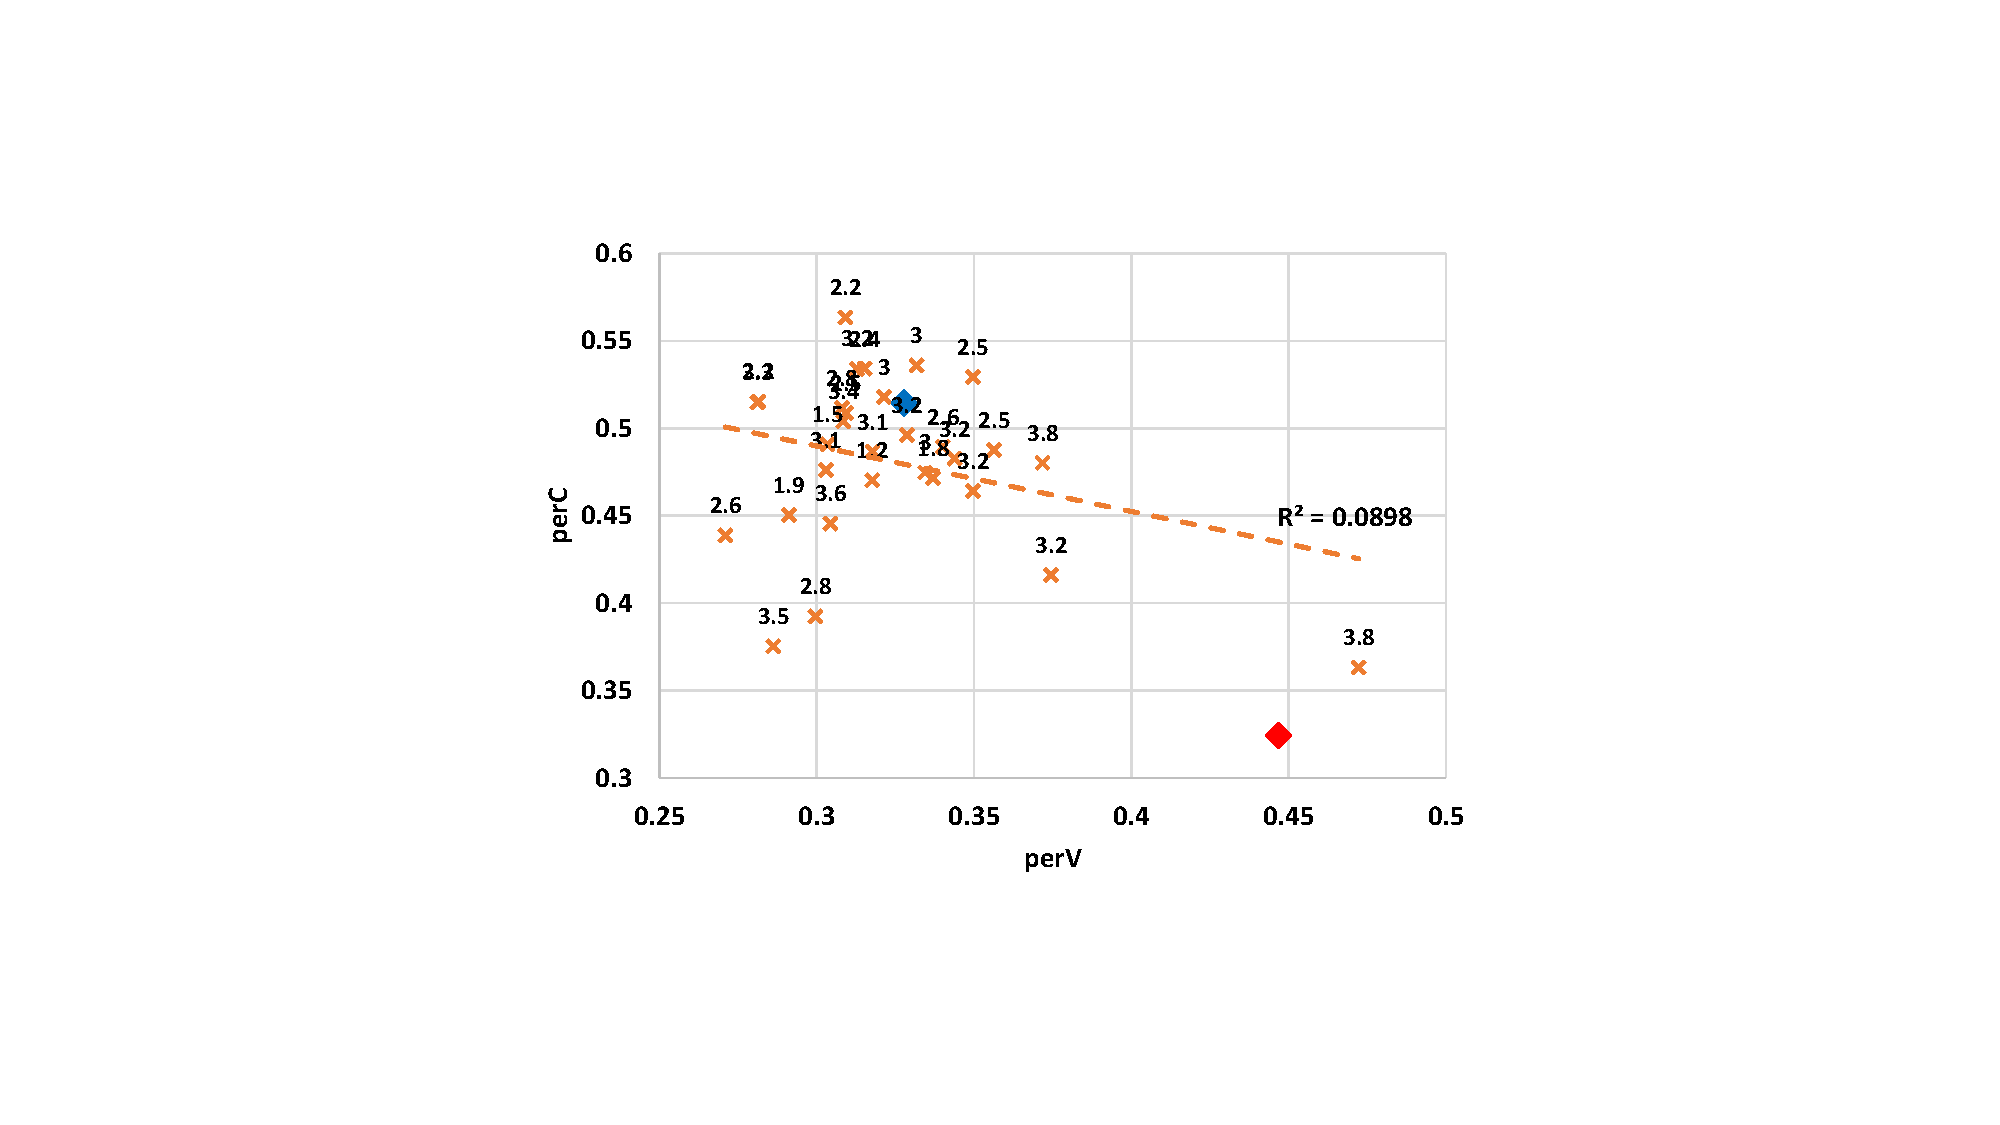
\includegraphics[width=5.0in]{figures/ch7_supraseg.pdf}
        \end{minipage}%
        \caption{Scatter plot of two rhythmic measurements of accented speech by Mandarin speakers: percentage of vocalic (X-axis) and consonantal (Y-axis) durations. The measurements of native English (Blue diamond) and Mandarin (Red diamond) are also shown.}
        \centering
        \label{fig:ch7_supraseg}
     \end{figure}

Figure \ref{fig:ch7_supraseg} demonstrates the scatter plot between two speech rhythmic measurements: the percentage of vocalic and consonantal durations extracted from Mandarin speakers. These two measurements are chosen because they show more L1's effect for strong accented speakers. X-axis is the percentage of vocalic duration (perV) and Y-axis is the percentage of consonantal duration (perC). Since these measurements are absolute values, both the values of L1, L2 and accented speech can be calculated independently. In the figure, the blue diamond is the position of native English; the red diamond is the position of native Mandarin; the orange crossings are accented speakers. The trend line (orange dash line) and R-square value are on the accented speakers only. Compared to English, Mandarin has high perV value but lower perC value. It can be found that measurements of most of accented speakers are around the native English, and only part of them are on the path from native L1 to native L2. This observation is in line with previous studies on L2 speech rhythm acquisition \citep{stockmal2005measures,lin2008interlanguage,li2014l2} where the authors show evidences that speech rhythmic measurements are not on the path from L1 to L2, indicating existence of effects that are independent from L1. However, the speaker with the highest accentedness score (3.8) clearly uses the L1 patterns to pronounce English. The results suggests that the prosodic patterns of accented speakers can be affected by L1, but may only influence a few prosodic dimensions or even be independent from L1; some speakers may not be affected by L1 prosodic patterns when producing L2 speech; speakers with mild accent also show no sign of being affected by L1 prosodic patterns.

To summarize, besides the conclusions drew by this study, it is expected that the methodology used in this study could facilitate further research directions on the interference of L1 in L2 speech learning process in a larger scale than previous studies. It can potentially reveal different factors that contribute to the perceived accentedness other than L1's effect. It can also benefit the L2 education field by individually giving a quantitative approximation of the process of L2 speech learning, and providing detailed feedback on which part of the English phonology the learners should focus on in following studies.

\section{Implication for practical computational models for speech applications}

Besides theoretical implications, this study can also contribute to the study on automatic accentedness evaluation. Automatic accentedness (or nativeness) evaluation plays an important role in computer-assisted pronunciation training (CAPT) and computer-aided language learning (CALL). State-of-the-art automatic system includes both the segmental and suprasegmental speech features to model the perception of foreign accent. However, they ignore the effect of L1 in L2 speech learning, and thus can be improved with the computational model proposed in this study. As already shown in chapter \ref{both_l1_l2}, adding the contrastive information between accented speech and L1 can improve the performance on accentedness prediction.

Another field that could benefit from the current study is speech intelligibility evaluation of pathological speech. This field is emerging as another important application area of speech technologies with the developing of telemedicine and increasing population impacted by speech disoreders. Although there is great interest in developing computational models for this application, current studies usually develops a feature extraction scheme or directly use existed feature extraction scheme such as Opensmile \citep{eyben2010opensmile}, and then build a machine learning model on the features as presented in my previous studies \citep{tu2016models,tu2017interpretable,tu2017objective}. The limitation is that existing feature extraction schemes for pathological speech only focus on low-level acoustic features directly calculated on time or frequency domain of original speech signal. This may be suboptimal when the machine learning model is not powerful enough or the amount of data is limited. As shown by \cite{tu2016relationship}, the performance of ASR have very strong correlation with the overall intelligibility of pathological speech. Thus, the computational model proposed in this study (without L1, and replace accented speech with pathological speech and accentedness with intelligibility or severity) can also be used for automatic evaluation of pathological speech.

However, a concern is that whether it is easy to obtain those L1 related features considering the need for a L1 acoustic model. In this study, L1 acoustic models trained on tens of or even over a hundred hours of speech recordings are employed. These L1 datasets may not be available in practice, especially for L1s with small amount of resources \citep{gales2017low}. Indeed, the pronunciation scores based features require acoustic models, but the acoustic models can be trained on small amount of data with phonemes as HMM modeling unit, thus reduce the model space and required training data. There is no need for large vocabulary ASR which usually requires much more speech data. Also, with a simpler acoustic model, the performance of forced-alignment will not be affected very much given known transcription of the accented speech.
